%% LyX 2.3.6.1 created this file.  For more info, see http://www.lyx.org/.
%% Do not edit unless you really know what you are doing.
\documentclass[english]{beamer}
\usepackage[T1]{fontenc}
\usepackage[latin9]{inputenc}
\setcounter{secnumdepth}{3}
\setcounter{tocdepth}{3}
\usepackage{amsbsy}
\usepackage{graphicx}

\makeatletter
%%%%%%%%%%%%%%%%%%%%%%%%%%%%%% Textclass specific LaTeX commands.
% this default might be overridden by plain title style
\newcommand\makebeamertitle{\frame{\maketitle}}%
% (ERT) argument for the TOC
\AtBeginDocument{%
  \let\origtableofcontents=\tableofcontents
  \def\tableofcontents{\@ifnextchar[{\origtableofcontents}{\gobbletableofcontents}}
  \def\gobbletableofcontents#1{\origtableofcontents}
}

%%%%%%%%%%%%%%%%%%%%%%%%%%%%%% User specified LaTeX commands.
%\usetheme{Warsaw}
\usetheme{CambridgeUS}
\usecolortheme{dolphin}

\setbeamertemplate{footline}{\hfill\insertframenumber/\inserttotalframenumber}
\defbeamertemplate*{footline}{shadow theme}
{%
  \leavevmode%
  \hbox{\begin{beamercolorbox}[wd=.5\paperwidth,ht=2.5ex,dp=1.125ex,leftskip=.3cm plus1fil,rightskip=.3cm]{author in head/foot}%
    \usebeamerfont{author in head/foot}
   \insertshortauthor
  \end{beamercolorbox}%

  \begin{beamercolorbox}[wd=.5\paperwidth,ht=2.5ex,dp=1.125ex,leftskip=0.5cm,rightskip=.3cm plus1fil]{title in head/foot}%
    \usebeamerfont{title in head/foot}\insertshorttitle% 
    \hskip45pt
    \insertframenumber\,/\,\inserttotalframenumber %\hfill
  \end{beamercolorbox}}%
  \vskip0pt%
}
\setbeamertemplate{navigation symbols}{} %no nav symbols

\usepackage{algpseudocode}
% Make vector print in bold
\renewcommand{\vec}[1]{\mbox{\boldmath$#1$}}

\makeatother

\usepackage{babel}
\begin{document}
\title[Jacob Jones]{A Comparative Study of $h$- and $p$- Geometric-Refinement of Curved Boundaries in      High-Order Finite and Spectral Element Methods}

\author[Jacob Jones]{Jacob Jones}

\institute{Stony Brook University \and Institute for Advanced Computational Science}

\date{June 21, 2023}

\begin{frame} 
 \titlepage 
\end{frame}
\begin{frame}{Outline}

\tableofcontents{}
\end{frame}


\section{Background and Skills}
\begin{frame}{Outline}

\tableofcontents[currentsection]
\end{frame}
%
\begin{frame}{Backgorund}
\begin{itemize}
\item B.S in Mathematics, SUNY college at old Westbury (2014 - 2018).
\item M.S in Applied Mathematics, Stony Brook University (2019 - 2020).
\item PhD in Applied Mathematics, Stony Brook University (2021 - 2024 expected).
\item Current research involves studying and developing code using hybrid
methods to solve PDEs numerically and study the impact of geometric
accuracy on numerical solutions.
\item Have a deep love and curiosity for mesh generation, mesh data structures,
and computational geometry.
\end{itemize}
\end{frame}
%
\begin{frame}{Skills}
\begin{itemize}
\item Taken courses featuring Numerical Linear Algebra, Scientific Computing,
Finite Difference Method, Finite Element Method, ODE's, PDE's
\item Experience programming in MATLAB, Python, C/C++.
\item Some experience with Mathematica, Fortran 90.
\item Familiar with modern programming standards and practices.
\item Familiar with modern programming workflow (GitHub, GitLab, Bitbucket
pull requests, branches, merging, etc.).
\end{itemize}
\end{frame}
%
\begin{frame}{Skills}
\begin{itemize}
\item Experience with High Performance Computing (MPI and OpenMP).
\item Experience with Data Structures.
\item Experience with Discrete Geometric Representation (Splines, Bezier
curves, NURBS).
\end{itemize}
\end{frame}

\section{Research}
\begin{frame}{Outline}

\tableofcontents[currentsection]
\end{frame}

\begin{frame}{Research Introduction}
\begin{itemize}
\item Spectral element methods (SEM) are extensions of finite element methods
(FEM) using Gauss-Lobatto or similar nodes instead of equidistant
nodes for high-order elements\footnote{Karniadakis and Sherwin. Spectral/hp Element Methods for Computational
Fluid Dynamics. (OUP Oxford, 2005).}.
\item Well-shaped tensor-product elements can deliver higher accuracy than
equidistant FEM due to potential superconvergence in the $\ell_{2}$-norm.
(nodal solutions)\footnote{Chen and Huang. High Accuracy Theory of Finite Elements (in Chinese).
(Hunan Science and Technique Press, Changsha, 1995).}
\item Significant challenges remain for domains with curved boundaries,
limiting the advantages of SEM for some real-world applications.
\end{itemize}
\end{frame}
%
\begin{frame}{Research Introduction}
\begin{itemize}
\item There has been significant evidence in isogeometric analysis\footnote{Hughes, Cottrell, and Bazilevs, Isogeometric analysis: CAD, finite
elements, NURBS, exact geometry and mesh refinement, Comput. Methods.
Appl. Mech. Eng. 194, 39-41 (2005), pp. 4135-{}-4195.} and NURBS-enhanced FEM (NEFEM)\footnote{Sevilla, Fern�ndez-M�ndez, Huerta. NURBS-enhanced finite element method
(NEFEM). Int. J. Numer. Methods. Eng. 76, 1 (2008), pp. 56-{}-83.} that a more accurate boundary representation can significantly improve
the overall accuracy of the solutions
\item Non-tensor-product elements (triangles/tets) are typically used near
boundaries, leading to the loss of superconvergence of the overall
solution.
\end{itemize}
\end{frame}

\begin{frame}{Example Problem}

\begin{center}
\begin{minipage}[t]{0.5\columnwidth}%
\begin{itemize}
\item Convection-Diffusion Equation $-\Delta u+\boldsymbol{v}\cdot\boldsymbol{\nabla}u=f$
\item Dirichlet boundary conditions on the straight boundaries
\item Neumann boundary conditions on the curved boundaries
\item Tested using manufactured solution
\end{itemize}
%
\end{minipage}\hspace{0.03\textwidth}%
\begin{minipage}[t]{0.2\columnwidth}%
\vspace{0.5cm}
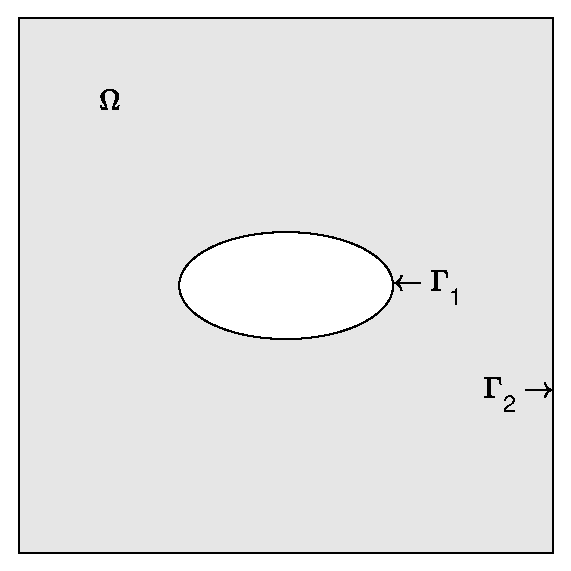
\includegraphics[scale=0.25]{../../speaf_paper/figures/domain_square_ellipse}
\begin{center}
Elliptical Hole Domain
\par\end{center}%
\end{minipage}\hspace{0.02\textwidth}%
\begin{minipage}[t]{0.2\columnwidth}%
\vspace{0.5cm}
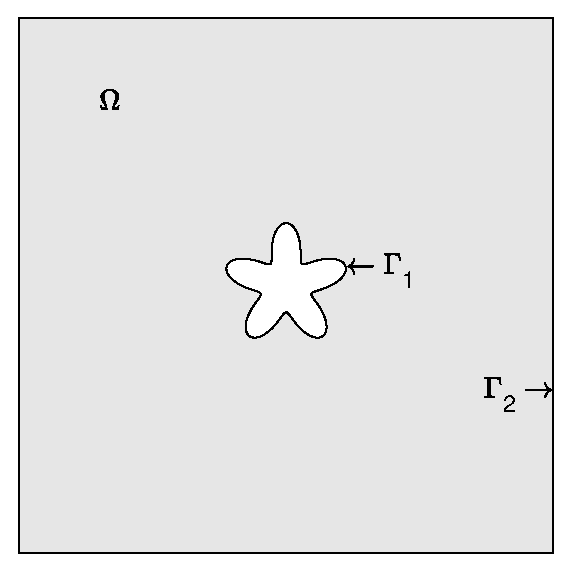
\includegraphics[scale=0.25]{../../speaf_paper/figures/domain_square_flower}
\begin{center}
Flower Hole Domain
\par\end{center}%
\end{minipage}
\par\end{center}

\end{frame}
%
\begin{frame}{Solution Approach}

\begin{itemize}
\item Novel approach to improve the overall accuracy and preserve the superconvergence
of SEM over curved domains.\footnote{\textbf{Jones}, Conley, \& Jiao. Preserving Superconvergence of Spectral
Elements for Curved Domains via $h$- and $p$- Geometric Refinement.
arxiv.org/abs/2304.13766}
\item Create a mesh using $h$- and $p$-geometric refinement:
\begin{itemize}
\item To apply $h$-geometric refinement, we generate a local edge length
$h$ at each node on the boundary, which is linearly related to the
curvature of the boundary,
\item To apply $p$-geometric refinement, we use superparemetric elements
on boundary elements, i.e., the degree of the geometric basis functions
is greater than the degree of the trial space.
\end{itemize}
\item Resolve the PDE using \textit{Adaptive Extended Stencil Finite Element
Method} (AES-FEM)\footnote{Conley, Delaney, \& Jiao. Overcoming element quality dependence of
finite elements with adaptive extended stencil FEM (AES-FEM). Int.
J. Numer. Meth. Engng., 2016.} on a decomposed subdomain near the curved boundary as a post-processing
step to reduce error and improve convergence.
\end{itemize}
\end{frame}
%
\begin{frame}{Summary of Post Processing AES-FEM}
\begin{itemize}
\item AES-FEM which combines features of the finite element method and the
generalized finite difference method.
\begin{itemize}
\item Use the traditional FEM linear `hat functions' as the weight functions.
\item Use \textit{Generalized Lagrange Polynomial Basis Functions} \textit{(GLPBF)},
which are calculated using a weighted-least squares approximation.
\end{itemize}
\item AES-FEM is not dependent on element quality and can achieve high-order
accuracy using linear meshes due to the fact that it is based on weighted
least squares.
\item Matrix assembly done in a \emph{Generalized Finite Difference (GFD)}-style
(node by node) allowing for easy parallelization without mesh partitioning.
\item Nodal Assembly requires each node has local element stencils.
\end{itemize}
\end{frame}
%
\begin{frame}{Initial Linear Mesh Setup}
\begin{itemize}
\item Generate mixed-element meshes using tensor-product elements in the
interior with triangular elements near curved boundaries.
\begin{itemize}
\item Generate a uniform quadrilateral mesh to cover the bounding box of
the domain.
\item Tag the nodes outside the computational domain or within some fixed
distance of a curved boundary.
\item Remove tagged nodes along with any quadrilateral containing them.
\item Mesh the gap between these edges and the curved boundary using an
off-the-shelf mesh generator.
\item Element connectivity table is built using the half-facet array algorithm\footnote{Dyedov, Ray, Einstein, Jiao, and Tautges, AHF: Array-based half-facet
data structure for mixed-dimensional and non-manifold meshes, Eng.
Comput. 31 (2015), pp. 389-{}-404.}.
\end{itemize}
\end{itemize}
\end{frame}

\begin{frame}{Generating the Initial Linear Mesh}

\begin{center}
\begin{minipage}[t]{0.27\columnwidth}%
\begin{center}
{\scriptsize{}Initial structured mesh and curved boundary $\Gamma$}{\scriptsize\par}
\par\end{center}
\begin{center}
\includegraphics[width=1\columnwidth]{../../speaf_paper/figures/initialmesh1}
\par\end{center}%
\end{minipage}\hspace{0.05\textwidth}%
\begin{minipage}[t]{0.27\columnwidth}%
\begin{center}
{\scriptsize{}After removing elements outside or on $\Gamma$}{\scriptsize\par}
\par\end{center}
\begin{center}
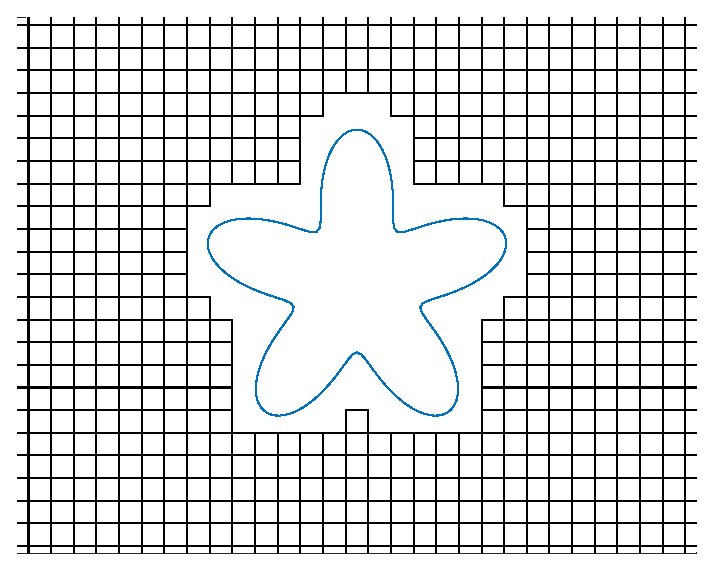
\includegraphics[width=1\columnwidth]{../../speaf_paper/figures/initialmesh2}
\par\end{center}%
\end{minipage}\hspace{0.05\textwidth}%
\begin{minipage}[t]{0.27\columnwidth}%
\begin{center}
{\scriptsize{}After generating conformal triangles}{\scriptsize\par}
\par\end{center}
\begin{center}
\includegraphics[width=1\columnwidth]{../../speaf_paper/figures/initialmesh3}
\par\end{center}%
\end{minipage}
\par\end{center}

\end{frame}
%
\begin{frame}{Applying $h$-Geometric Refinement}
\begin{itemize}
\item Seek to generate a local edge length $h$ at each node on the boundary,
which is linearly related to the curvature of the boundary.
\item Evaluate the curvature for each node on the curved boundary using
either the explicit parameterization or some form of geometric reconstruction.
\item Define a target angle $\theta_{max}$ such that no two adjacent nodes
have a difference in the normal direction that is greater than $\theta_{max}$.
\item Make the target edge length the arc length of the circle defined by
the radius of curvature and $\theta_{max}$, $h_{i}=\theta_{max}R_{i}=\theta_{max}/K_{i}$.
\item Limit the minimum and maximum edge lengths using parameters $h_{min}$
and $h_{max}$.
\[
h_{i}=\mathrm{min}(\mathrm{max}(\theta_{max}/K_{i},h_{min}),h_{max})
\]
\end{itemize}
\end{frame}

\begin{frame}{Meshing with $h$-Geometric Refinement}

\begin{center}
\begin{minipage}[t]{0.45\columnwidth}%
\begin{center}
Without $h$-Geometric Refinement
\par\end{center}
\begin{center}
\includegraphics[width=1\columnwidth]{figures/CBRmesh1}
\par\end{center}%
\end{minipage}\hspace{0.05\textwidth}%
\begin{minipage}[t]{0.45\columnwidth}%
\begin{center}
With $h$-Geometric Refinement
\par\end{center}
\begin{center}
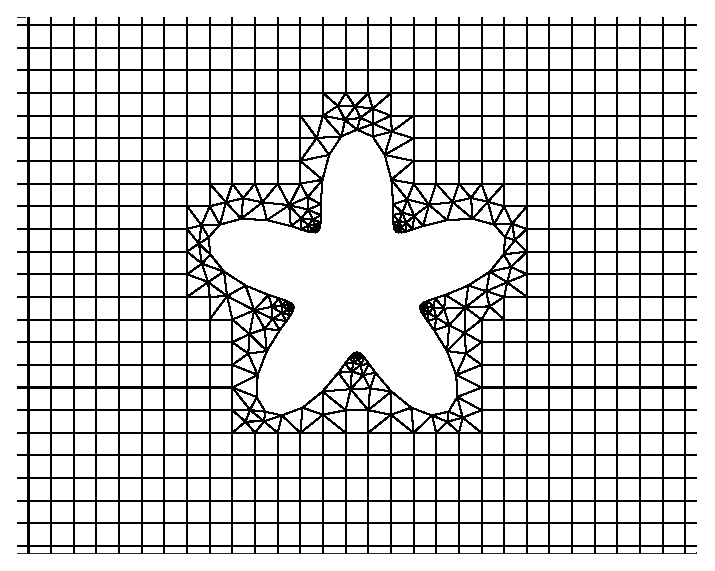
\includegraphics[width=1\columnwidth]{figures/CBRmesh2}
\par\end{center}%
\end{minipage}
\par\end{center}

\end{frame}
%
\begin{frame}{Applying $p$-Geometric Refinement}
\begin{itemize}
\item Superparametric elements\footnote{M Reza Eslami, Finite Elements Methods in Mechanics (Springer, 2014).}
on curved boundary.
\item Degree of the geometric basis functions is greater than the degree
of the trial space.
\item Helps to improve geometric accuracy on curved Neumann boundaries so
superconvergence can be recovered.
\end{itemize}
\end{frame}
%
\begin{frame}{Placing High Order Nodes}
\begin{itemize}
\item Insert mid-edge and mid-face nodes to generate high-order spectral
elements.
\item For the rectangular elements in the interior of the domain, we insert
Gauss-Lobatto points.
\item For the triangular, we use Gauss-Lobatto nodes for the facets (i.e.,
edges) shared between tensor-product and non-tensor-product elements
to ensure continuity.
\item For interior nodes we place them at quadrature points that maximize
the degree of the quadrature rule as Gauss-Lobatto points do.
\item If element has a curved edge, the placement of the nodes needs to
satisfy Ciarlet-Raviart condition\footnote{Ciarlet and Raviart, The combined effect of curved boundaries and
numerical integration in isoparametric finite element methods, The
Mathematical Foundations of the Finite Element Method with Applications
to Partial Differential Equations (Elsevier, 1972), pp. 409-{}-474.} to preserve the convergence rate.
\end{itemize}
\end{frame}
%
\begin{frame}{Placing High Order Nodes}
\begin{itemize}
\item Ciarlet-Raviart condition requires the Jacobian determinant of a degree-$p$
element to have bounded derivatives up to $(p+1)$st order.
\item We use an iterative process similar to the one presented in \footnote{Li, Zhao, Ray, and Jiao, Compact feature-aware Hermite-style high-order
surface reconstruction, Eng. Comput. 37, 1 (2021), pp. 187-{}-210.}.
\item Found that the Jacobian determinant is sufficiently smooth to reduce
the pollution errors of the spectral elements.
\end{itemize}
\end{frame}
%
\begin{frame}{Extraction of Near Boundary Elements}
\begin{itemize}
\item To utilize AES-FEM near the boundary a linear mesh is required.
\item Construct a new, smaller, linear mesh by decomposing the high-order
mesh.
\item Choosing just decomposed triangles from original mesh will not be
sufficient to improve accuracy. 
\item Extension into the quadrilateral section of the mesh by a number of
layers is required.
\item A layer is defined as all quadrilaterals with two or more nodes as
part of the AES-FEM mesh.
\end{itemize}
\end{frame}
%
\begin{frame}{Extraction of Near Boundary Elements}

\begin{minipage}[t]{0.45\columnwidth}%
\begin{center}
Quadratic mesh before splitting
\par\end{center}
\begin{center}
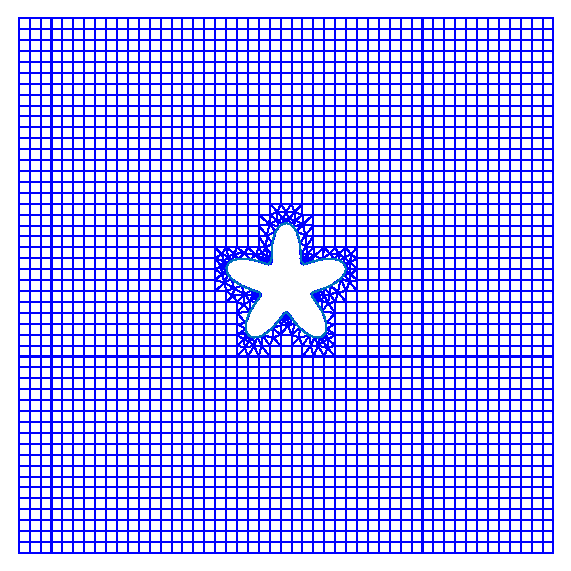
\includegraphics[width=1\columnwidth]{../../speaf_paper/figures/aes_fem_extract_mesh}
\par\end{center}%
\end{minipage}\hspace{0.05\textwidth}%
\begin{minipage}[t]{0.45\columnwidth}%
\begin{center}
AES-FEM mesh after splitting
\par\end{center}
\begin{center}
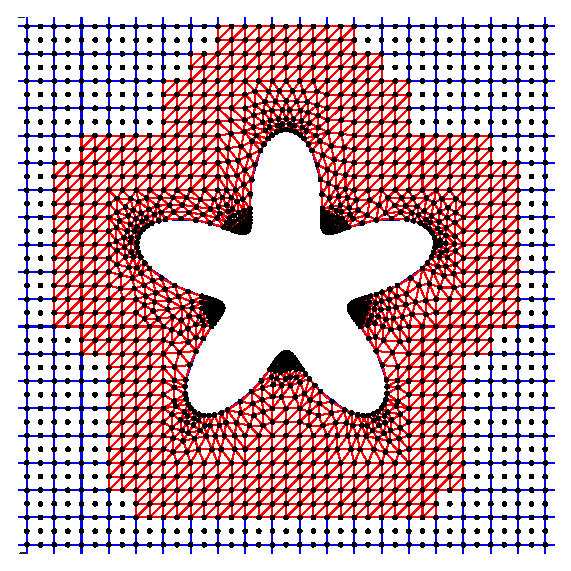
\includegraphics[width=1\columnwidth]{../../speaf_paper/figures/aes_fem_extract_mesh_zoomed}
\par\end{center}%
\end{minipage}
\end{frame}
%
\begin{frame}{$h$-Geometric Refinement Results}

\begin{minipage}[t]{0.45\textwidth}%
\begin{center}
\includegraphics[width=1\textwidth]{../../speaf_paper/figures/ell_cd_Quadratic_test_1}\\
{\scriptsize{}(a) Quadratic elliptical hole}
\par\end{center}%
\end{minipage} %
\begin{minipage}[t]{0.45\textwidth}%
\begin{center}
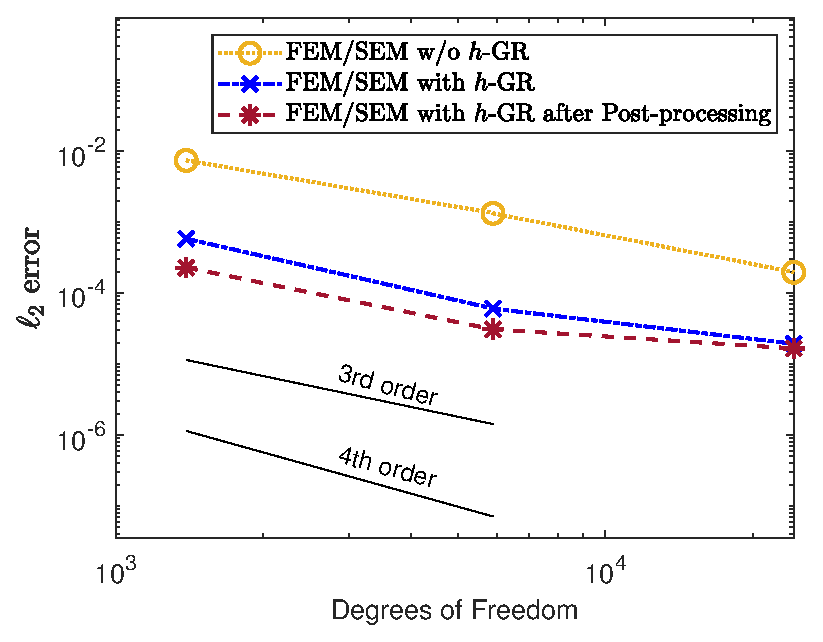
\includegraphics[width=1\textwidth]{../../speaf_paper/figures/flo_cd_Quadratic_test_1}\\
{\scriptsize{}(b) Quadratic flower hole}
\par\end{center}%
\end{minipage}
\end{frame}
%
\begin{frame}{$h$-Geometric Refinement Results}

\begin{minipage}[t]{0.45\textwidth}%
\begin{center}
\includegraphics[width=1\textwidth]{../../speaf_paper/figures/ell_cd_Cubic_test_1}\\
{\scriptsize{}(c) Cubic elliptical hole}
\par\end{center}%
\end{minipage} %
\begin{minipage}[t]{0.45\textwidth}%
\begin{center}
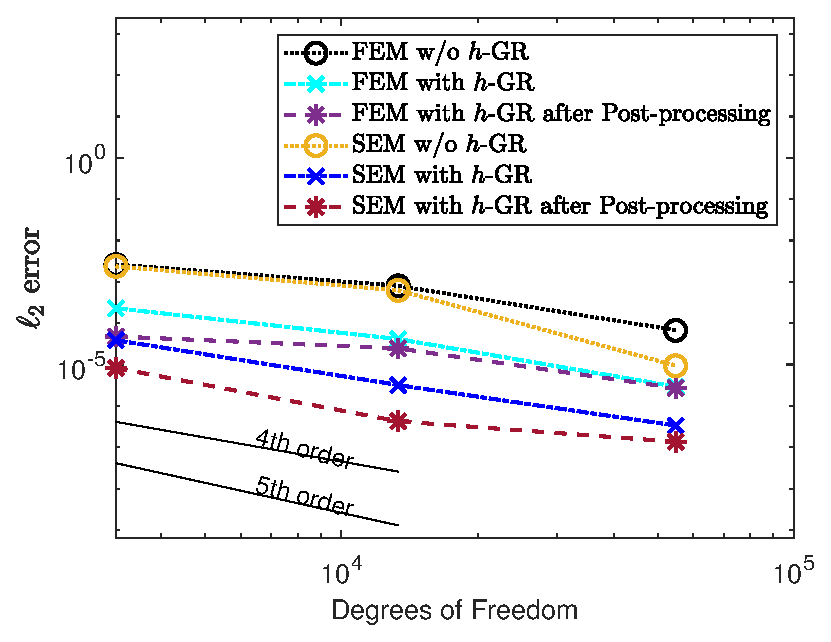
\includegraphics[width=1\textwidth]{../../speaf_paper/figures/flo_cd_Cubic_test_1}\\
{\scriptsize{}(d) Cubic flower hole}
\par\end{center}%
\end{minipage}
\end{frame}
%
\begin{frame}{$h$-Geometric Refinement Results}

\begin{minipage}[t]{0.45\textwidth}%
\begin{center}
\includegraphics[width=1\textwidth]{../../speaf_paper/figures/ell_cd_Quartic_test_1}\\
{\scriptsize{}(e) Quartic elliptical hole}
\par\end{center}%
\end{minipage} %
\begin{minipage}[t]{0.45\textwidth}%
\begin{center}
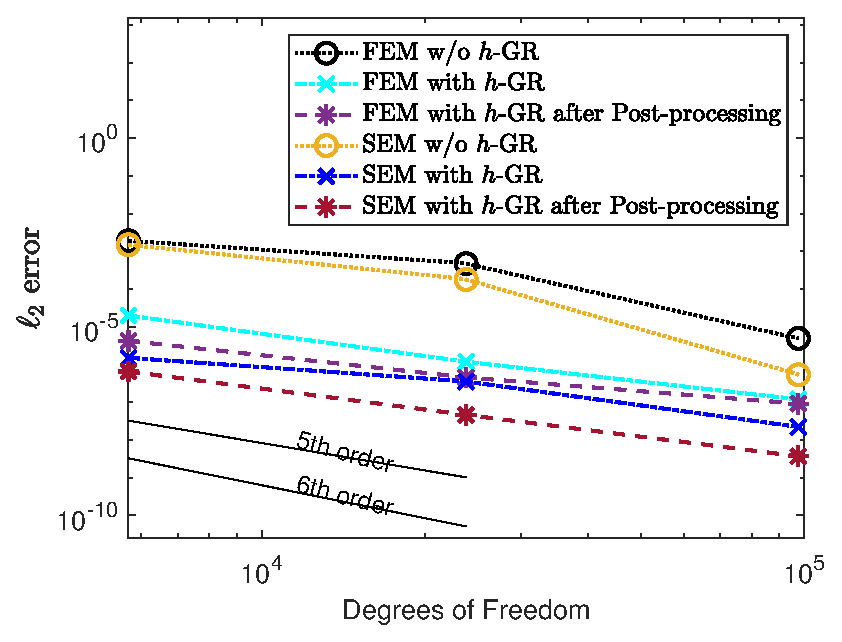
\includegraphics[width=1\textwidth]{../../speaf_paper/figures/flo_cd_Quartic_test_1}\\
{\scriptsize{}(f) Quartic flower hole}
\par\end{center}%
\end{minipage}
\end{frame}
%
\begin{frame}{$hp$-Geometric Refinement Results}

\begin{minipage}[t]{0.45\textwidth}%
\begin{center}
\includegraphics[width=1\textwidth]{../../speaf_paper/figures/ell_cd_Quartic_test_2}\\
{\scriptsize{}(e) Quartic elliptical hole}
\par\end{center}%
\end{minipage} %
\begin{minipage}[t]{0.45\textwidth}%
\begin{center}
\includegraphics[width=1\textwidth]{../../speaf_paper/figures/flo_cd_Quartic_test_2}\\
{\scriptsize{}(f) Quartic flower hole}
\par\end{center}%
\end{minipage}
\end{frame}
%
\begin{frame}{Future Work}
\begin{itemize}
\item Generate high-order hybrid meshes in 3D with curved boundary elements.
\item More formally present post-processing method and show superconvergent
results in 3D.
\item Show that AES-FEM near the boundary adds only minimum extra computation
to the overall workflow.
\end{itemize}
\end{frame}
%
\begin{frame}{My Contributions}
\begin{itemize}
\item Writing all of the meshing and geometry code.
\item Writing code to compute local nodal stencils in 2D and 3D (used for
GFD and AES-FEM).
\item Writing code to assemble finite/spectral element stiffness matrices
with Dirichlet and Neumann boundary conditions.
\item Writing all code to assemble GFD and AES-FEM stiffness matrices with
Dirichlet and Neumann boundary conditions in parallel using OpenMP.
\item Writing all code to assemble local Vandermode matrices for GFD in
2D and 3D.
\item Writing all code to perform the hybrid method, transferring solutions
from SEM to AES-FEM.
\end{itemize}
\end{frame}


\section{Mesh Generation}
\begin{frame}{Outline}

\tableofcontents[currentsection]
\end{frame}
%
\begin{frame}{Mesh Generation}
\begin{itemize}
\item Enjoy writing mesh generation software for fun.
\item Experience in Delaunay Triangulation / Tetrihedrization.
\item Familiar with Delaunay point insertion algorithms.
\item Familiar with Delaunay refinement algorithms (Ruppert, Chews second,
etc).
\item Developed my own refinement algorithm for fun based on Chews second
algorithm.
\item Familiar with nodal smoothing techniques to improve mesh quality.
\item Familiar with mesh partitioning
\end{itemize}
\end{frame}
%
\begin{frame}{Mesh Generation}

\begin{center}
\begin{minipage}[t]{0.45\columnwidth}%
\begin{center}
\includegraphics[width=1\columnwidth]{figures/monalisa}
\par\end{center}%
\end{minipage}%
\begin{minipage}[t]{0.45\columnwidth}%
\begin{center}
\includegraphics[width=1\columnwidth]{figures/Flower}
\par\end{center}%
\end{minipage}
\par\end{center}

\end{frame}


\section{Current Work at LANL}
\begin{frame}{Outline}

\tableofcontents[currentsection]
\end{frame}
%
\begin{frame}{Remap}
\begin{itemize}
\item Need to transfer quantity from one mesh to another while maintaining
some conservative property.
\item Need to find geometry of the overlapping region (overlap between elements).
\end{itemize}
\begin{center}
\begin{minipage}[t]{0.45\columnwidth}%
\begin{center}
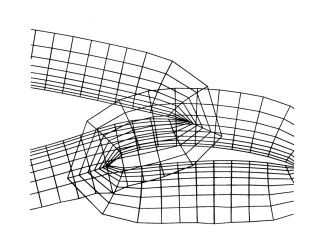
\includegraphics[width=1\columnwidth]{figures/OverlappingDiagram_sm}
\par\end{center}%
\end{minipage}
\par\end{center}

\end{frame}
%
\begin{frame}{Tet-Tet Overlap}
\begin{itemize}
\item In a mesh of Hexahedrals, consider two overlapping elements.
\item The source Hexahedral is decomposed into 24 Tetrahedra (to account
for non-coplanar quadrangle faces).
\item Currently \textbf{r3D}\footnote{Powell, D. r3d: Software for fast, robust geometric operations in
3D and 2D. Report of Los Alamos national laboratory, LA-UR-15-26964.
Report and software are available at https://github. com/devonmpowell/r3d
(2015).} is applied to each Tetrahedra and a Clip and Cap algorithm is used
to find the overlap geometry with the target Hexahedra but has significant
computational cost.
\item If instead both Hexahedrals are decomposed then we can consider only
Tet-Tet overlaps.
\item Objective is to find a fast, array based algorithm to perform specifically
Tet-Tet overlaps.
\item Eventual goal is to port fast algorithm to GPUs.
\end{itemize}
\end{frame}
%
\begin{frame}{Thank you}

\vspace{2cm}

\begin{center}
{\Huge{}Thank you!}\vspace{2cm}
\par\end{center}

\end{frame}


\end{document}
